% !TEX root = ../diz.tex
\begin{veta}
  Any maximal parallel P system with cooperative rules without dissolution can be simulated by a sequential P system with cooperative rules and inhibitors.
\end{veta}

\begin{dokaz}
  We show that we can simulate a step of the maximal parallel P system with several steps of a sequential P system with inhibitors.

  % Membrane states

  It is important to note that in the maximal parallel step the evolution occurs simultaneously in all membranes, so we need to synchronize this process.
  The steps of the sequential P system simulating the maximal parallel step are divided into several phases. Every membrane will have a phase, represented as an object. There is exactly one phase object in each membrane. 

  The $\mathit{RUN}$ phase represents that the rules of the maximal parallel P system are being applied, one-by-one. When there are no more rules to apply, the membrane has done its maximal parallel step and proceeds to the phase $\mathit{SYNCHRONIZE}$. Other phases are just technical - we need to implement sending objects between membranes and preparing for the next maximal parallel step by unmarking newly created objects in the current maximal parallel step, which have been marked to prevent double evolution in one step.

  \begin{itemize}
    \item $\mathit{\bf RUN}$: Rules of the maximal parallel P system are being applied. Products are marked ($a^\prime$ instead of $a$) in order to prevent further evolution in the same maximal parallel step. Objects that are to be sent to the parent membrane are directly sent because the parent membrane is in $\mathit{RUN}$ or $\mathit{SYNCHRONIZE}$ phase (see figure \ref{fig:possible_pairs_of_states_of_parent_and_child_membrane}), so the $a^{\prime}$ symbols that are sent will not be used in any rule until phase $\mathit{RESTORE}$. But objects that are to be sent down to child membrane $l$, cannot be sent immediately because membrane $l$ can be in the previous phase waiting to restore symbols from previous step. Objects $a^\prime$ could interfere with them resulting in double application in current maximal parallel step. Such objects are only marked as $a^{\downarrow_l\prime}$ to be sent down in the phase $\mathit{SENDDOWN}$. When the phase $\mathit{RUN}$ ends, next phase $\mathit{SYNCHRONIZE}$ takes place, while emitting an object $\mathit{SYNCTOKEN}$ to the parent membrane with a purpose to deliver it to the skin membrane.

    \item $\mathit{\bf SYNCHRONIZE}$: There was no applicable rule left so the membrane is waiting to get signal $\mathit{SYNCED}$ from the parent membrane to proceed to the next phase. And also resending all $\mathit{SYNCTOKEN}$ objects to the parent membrane.

    \item $\mathit{\bf SENDDOWN}$: Signal $\mathit{SYNCED}$ was caught, which means that every membrane has already been in the $\mathit{SYNCHRONIZE}$ phase. And all descendant membranes are in $\mathit{SYNCHRONIZE}$ phase. In this phase all the objects $a^{\downarrow_l\prime}$ can be sent down.

    \item $\mathit{\bf RESTORE}$: All $a^{\prime}$ symbols are being restored to $a$, preparing for the next maximal parallel step.
  \end{itemize}

  % Objects

  We will now introduce the objects used in the simulation.
  
  \begin{itemize}
    \item The alphabet $\Sigma$ of the maximal parallel P system.
    \item $a^\prime$ for $a\in\Sigma$ used as products of a rule application waiting for the synchronization.
    \item $a^{\downarrow_l\prime}$ for $a\in\Sigma$ and $1\leq l\leq m$ used as products of a rule application which should be sent down to membrane $l$. 
    \item $\dot{a}$ for $a\in\Sigma$ can be used normally in rewriting, with a constraint to have at most one instance of $\dot{a}$ in a membrane. It helps with deciding presence of an applicable rule. 
    \item objects representing phases $\mathit{RUN}$, $\mathit{SYNCHRONIZE}$, $\mathit{SENDDOWN}$, $\mathit{RESTORE}$.
    \item $SYNCTOKEN_i$ for each membrane with label $i$ to let the skin membrane know the membrane $i$ is waiting in synchronization phase.
    \item $SYNCED$ used as a broadcast from the skin membrane to let each membrane know that each other membrane has already been synchronized.
    \item $NA_j$ meaning the rule $r_j$ is not applicable. There is at most one occurrence of $NA_j$ in a membrane.
  \end{itemize}

  At the start of the simulation the configuration of simulating sequential P system is the same as the configuration of the simulated maximal parallel P system, with a $\mathit{RUN}$ symbol in each membrane.

  % Rewriting rules

  We will now define the evolution rules in a membrane with label $i$ of the simulating P system.

  \begin{itemize}
    \item For every rule $r_j\in R_i$ such that
      \begin{align*}
        r_j = a_1^{M(a_1)}a_2^{M(a_2)}\dots a_n^{M(a_n)} \rightarrow b_1\dots b_x c_1\uparrow\dots c_y\uparrow d_1\downarrow_{l_1}\dots d_z\downarrow_{l_z}
      \end{align*}
      we will have the following rules:
      \begin{align*}
        &a_1^{M(a_1)-m_1}\dot{a}_1^{m_1}
        a_2^{M(a_2)-m_2}\dot{a}_2^{m_2}\dots
        a_n^{M(a_n)-m_n}\dot{a}_n^{m_n}|\mathit{RUN} \\
        \rightarrow &b_1^\prime\dots b_x^\prime c_1^\prime\uparrow\dots c_y^\prime\uparrow d_1^{\downarrow_{l_1}\prime}\dots d_z^{\downarrow_{l_z}\prime}|\mathit{RUN}
      \end{align*}
      
      There will be such rule for each $0\leq m_k\leq min(M(a_k),1)$. It represents the idea that $\dot{a_k}$ can be used in rule application in the same way as $a_k$. The number of occurrences of $\dot{a_k}$ is 0 or 1. If $M(a_k) = 0$, the rule $r_j$ has no presence of $a_k$ on the left side so in this case we will have just rules where $m_k=0$. Right side of the rules contains symbols $a^\prime$, that prevents the symbols to be evolved again.

    \item For every object $a\in\Sigma$, in order to guarantee at most one occurrence of $\dot{a}$ in the membrane, we will have the following rule:
    $$a|\mathit{RUN} \rightarrow \dot{a}|\mathit{RUN}|_{\neg \dot{a}}$$

    \item For every rule $r_j\in R_i$ there will be a rule that detects if the rule $r_j$ is not applicable. If there is not enough objects present in the membrane to satisfy left side of the rule $r_j$, object $\mathit{NA_i}$ is created.

    If the left side of the rule $r_i$ is of type:
    \begin{itemize}
      \item $a$: It is a context free rule. This rule cannot be applied iff there is no occurrence of $a$ nor $\dot{a}$.
        $$\mathit{RUN} \rightarrow \mathit{NA_j}|\mathit{RUN}|_{\neg\{\mathit{NA_j}, a, \dot{a}\}}$$
      \item $ab$: It is a cooperative rule with two distinct objects on the left side. This rule cannot be applied iff there is one of them missing.
        \begin{align*}
          &\mathit{RUN} \rightarrow \mathit{NA_j}|\mathit{RUN}|_{\neg\{\mathit{NA_j}, a, \dot{a}\}}\\
          &\mathit{RUN} \rightarrow \mathit{NA_j}|\mathit{RUN}|_{\neg\{\mathit{NA_j}, b, \dot{b}\}}
        \end{align*}
      \item $a^2$: It is a cooperative rule requiring presence of two instances of an object. This rule cannot be applied iff there is at most one occurrence of the object. That happens iff there is no occurrence of $a$. There can still be $\dot{a}$, but at most one occurrence.
        $$\mathit{RUN} \rightarrow \mathit{NA_j}|\mathit{RUN}|_{\neg\{\mathit{NA_j}, a\}}$$
    \end{itemize}

    \item A rule detecting the maximal set of rules has been applied and no further rule is applicable:
    \begin{align*}
      &\mathit{NA_1}|\mathit{NA_2}|\dots|\mathit{NA_{|R_i|}}|\mathit{RUN} \\
      \rightarrow &\mathit{SYNCHRONIZE}|\mathit{SYNCTOKEN_i}
    \end{align*}

    If no additional rule can be applied, the simulation of a maximal parallel step in the membrane is complete and it waits for other membranes to complete their maximal parallel step.

    \item Membrane $i>1$ (different from the skin membrane) resends synchronization token originating from any membrane $l$ to the parent membrane with a purpose of deliver it to the skin membrane:
    \begin{align*}
      &\mathit{SYNCHRONIZE}|\mathit{SYNCTOKEN_l} \\
      \rightarrow &\mathit{SYNCHRONIZE}|\mathit{SYNCTOKEN_l}\uparrow
    \end{align*}

    \item In the skin membrane ($i=1$) there is a rule which collects synchronization tokens from all membranes $1\dots p$ and then executes the phases $\mathit{SENDDOWN}$ and $\mathit{RESTORE}$ after which it sends down signal that synchronization is complete.
    \begin{align*}
      &\mathit{SYNCTOKEN_1}|\dots|\mathit{SYNCTOKEN_p}|\mathit{SYNCHRONIZE} \\
      \rightarrow &\mathit{SENDDOWN}
    \end{align*}

    \item Every membrane other than skin membrane ($i>1$) is waiting for the $\mathit{SYNCED}$ signal to go to the $\mathit{SENDDOWN}$ phase:
    $$\mathit{SYNCHRONIZE}|\mathit{SYNCED} \rightarrow \mathit{SENDDOWN}$$

    \item Every membrane will have rules to send down all objects prepared to be sent down $a^{\downarrow_l\prime}$, where $a\in \Sigma$ and $1\leq l\leq m$:
    $$\mathit{SENDDOWN}|a^{\downarrow_l\prime} \rightarrow \mathit{SENDDOWN}|a^{\prime}\downarrow_l$$

    \item Every membrane will have a rule for detecting when all such objects have been sent down in order to proceed to the $\mathit{RESTORE}$ phase:
    $$\mathit{SENDDOWN} \rightarrow \mathit{RESTORE}|_{\neg \{a^{\downarrow_l\prime}|a\in\Sigma, 1\leq l\leq m\}}$$

    \item In the $\mathit{RESTORE}$ phase all objects $a^{\prime}$ will be evolved to $a$ so it can be evolved in the next maximal parallel step:
    $$\mathit{RESTORE}|a^{\prime} \rightarrow \mathit{RESTORE}|a$$

    \item Descendant membranes are waiting for the signal $\mathit{SYNCED}$, which is sent to all direct child membranes $l_1\dots l_z$ when the $\mathit{RESTORE}$ phase ends. It also means that the next maximal parallel step is already being simulated in the ancestor membranes ($\mathit{RUN}$ or $\mathit{SYNCHRONIZE}$ phase):
    $$\mathit{RESTORE} \rightarrow \mathit{RUN}|\mathit{SYNCED}\downarrow_{l_1}|\dots|\mathit{SYNCED}\downarrow_{l_z}|_{\neg \{a^{\prime}|a\in\Sigma\}}$$
  \end{itemize}

  \definecolor{run}{rgb}{1,0.5,0}
  \definecolor{restore}{rgb}{0,0.5,0}
  \definecolor{synchronize}{rgb}{0,0,1}
  \definecolor{senddown}{rgb}{1,0,0}
  % Narrow texts in boxes
  \providecommand{\narrow}[1]{\scalebox{.85}[1.0]{#1}}

  \begin{figure}
    \def\svgwidth{\textwidth}
    \input{possible_pairs_of_states_of_parent_and_child_membrane.pdf_tex}
    % 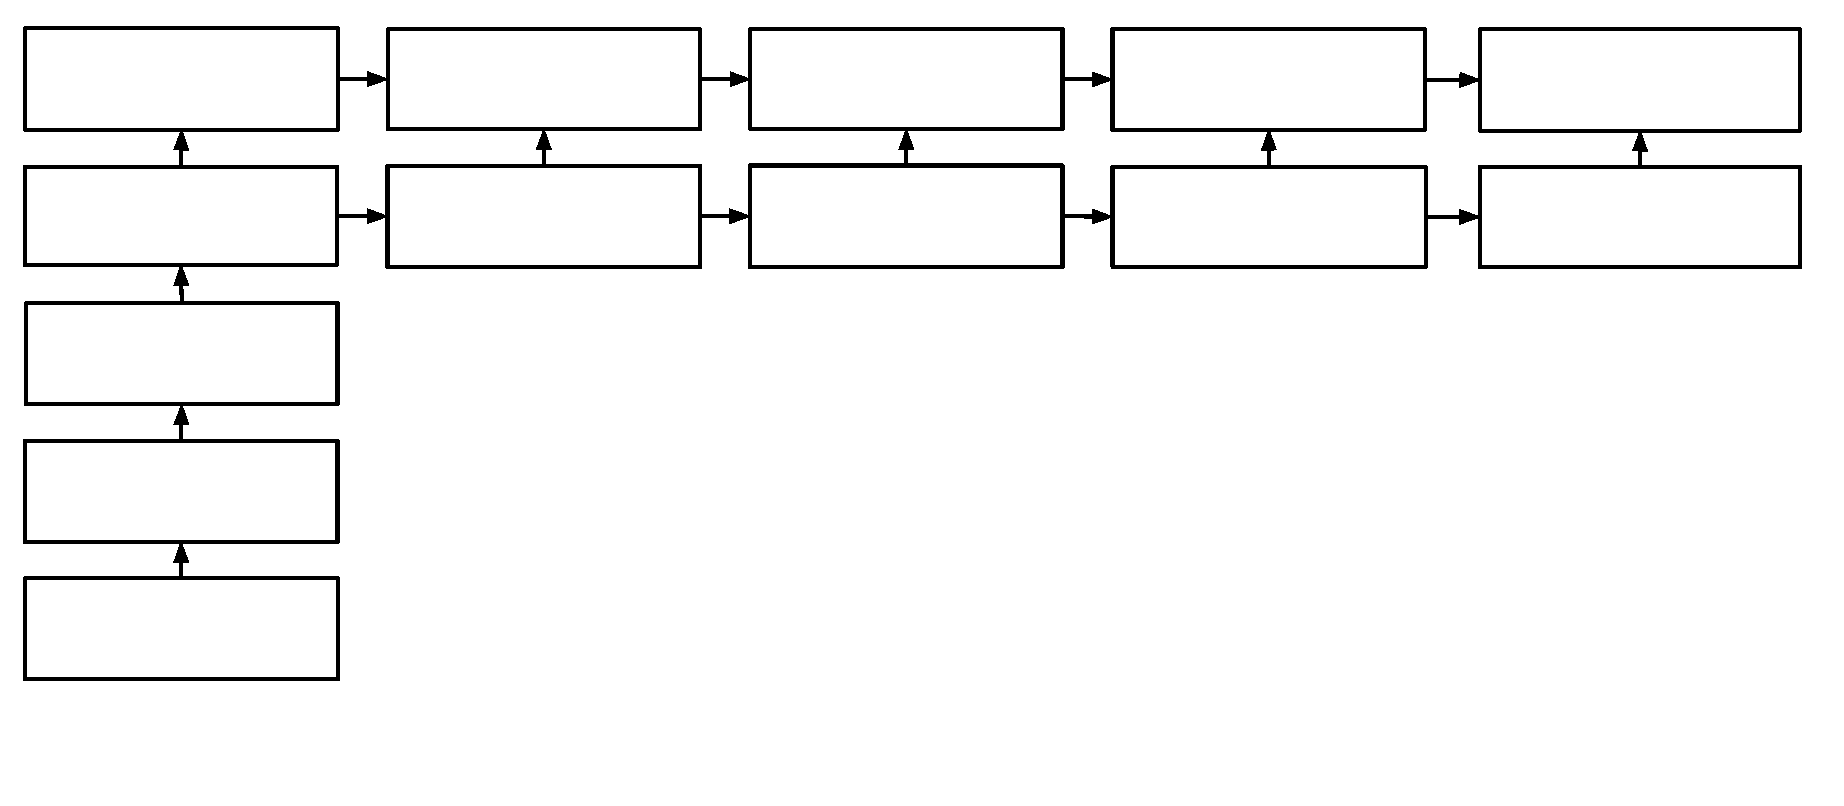
\includegraphics[width=\textwidth]{possible_pairs_of_states_of_parent_and_child_membrane}
    \caption{Possible pairs of states of parent and child membrane}
    \label{fig:possible_pairs_of_states_of_parent_and_child_membrane}
  \end{figure}

  \begin{figure}
    \def\svgwidth{\textwidth}
    \input{snapshot_of_all_membrane_states_while_simulating.pdf_tex}
    % 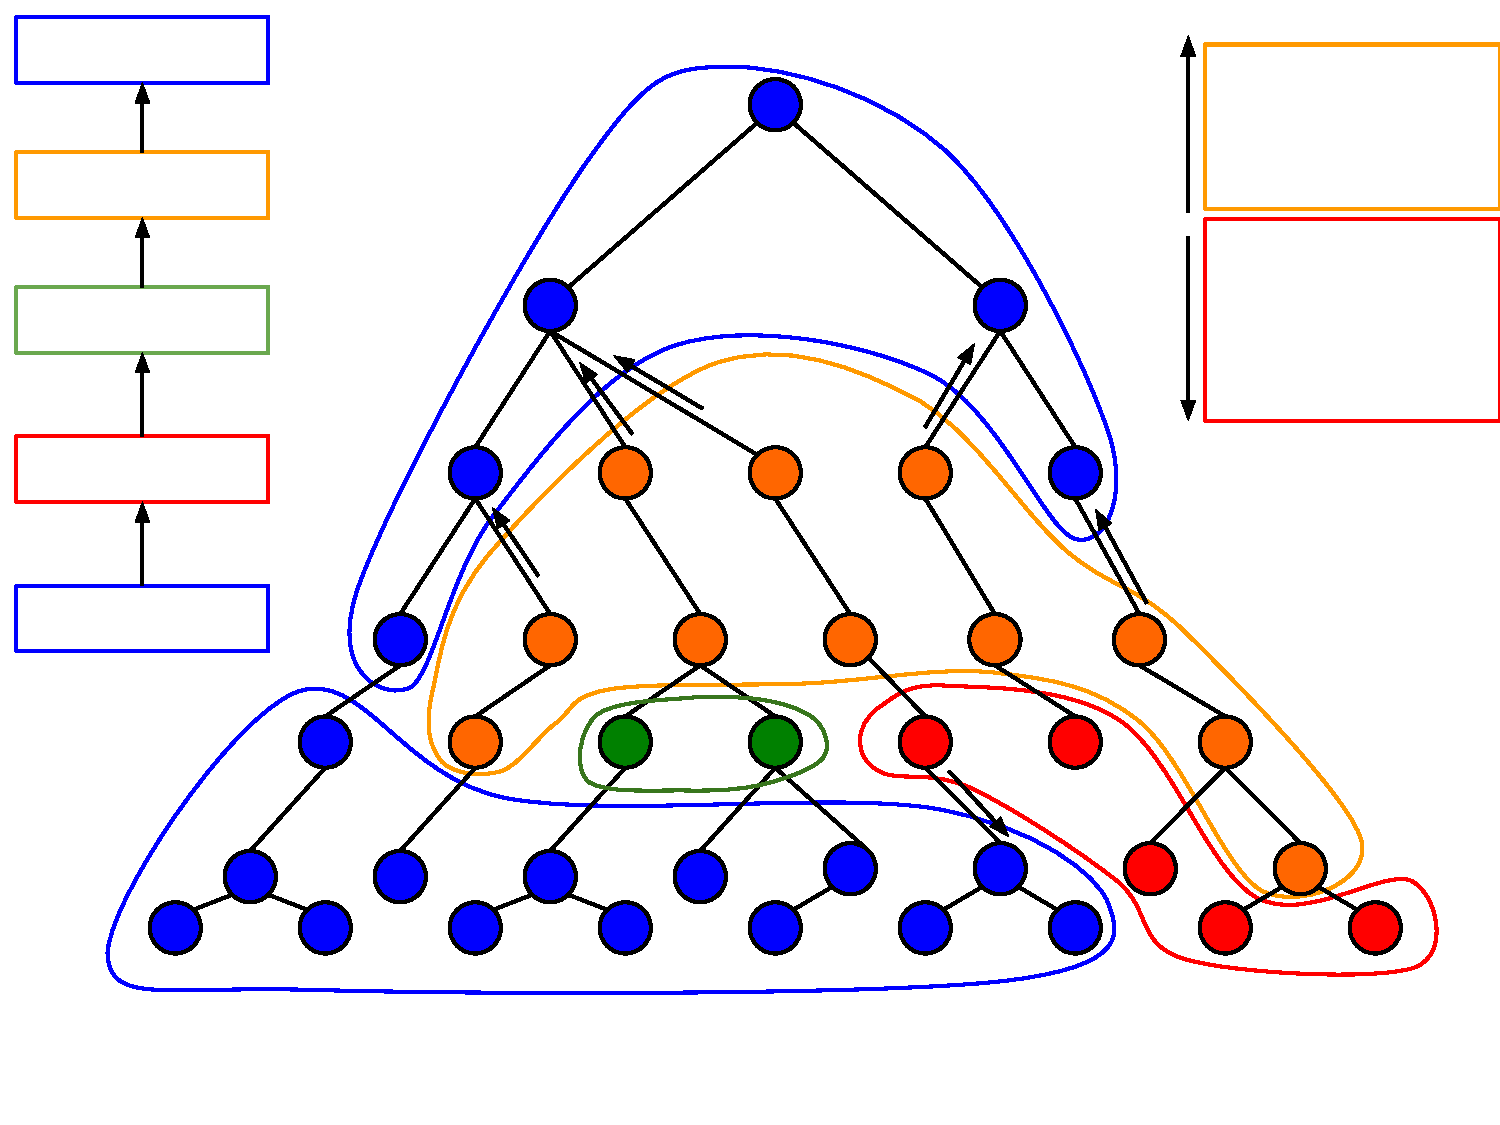
\includegraphics[width=\textwidth]{snapshot_of_all_membrane_states_while_simulating}
    \caption{Snapshot of all membrane states while simulating}
    \label{fig:snapshot_of_all_membrane_states_while_simulating}
  \end{figure}

  The pairs of possible phases of the parent and child membrane are shown in the figure \ref{fig:possible_pairs_of_states_of_parent_and_child_membrane} along with transitions between two consecutive global synchronizations - after the maximal parallel steps $i$ and $i+1$.

  In the figure \ref{fig:snapshot_of_all_membrane_states_while_simulating} the membrane structure is presented as a hierarchical structure. Every membrane is in one of four phases. It can be seen that the sending of the objects is performed in such phases that the receiving membrane is in either $\mathit{RUN}$ or $\mathit{SYNCHRONIZE}$ phase, so the received objects (marked $a^\prime$) does not interfere with rewriting.

  Another interesting idea can be seen in the figure \ref{fig:snapshot_of_all_membrane_states_while_simulating} that when a region is in the $\mathit{SENDDOWN}$ phase and objects are sent through the child membrane, the receiving region is in the $\mathit{SYNCHRONIZE}$ phase waiting for the $\mathit{SYNCED}$ signal, which will be sent to it when $\mathit{SENDDOWN}$ and $\mathit{RESTORE}$ phases finished. \qed

\end{dokaz}

It is even possible to define a \index{Bisimulation!branching}branching bisimulation between states of the two P systems in the simulation above. We define:
\begin{enumerate}
  \item a labeled transition system $L_1$ for simulated maximal parallel P systems
  \item a labeled transition system with silent actions $L_2$ for simulating sequential P system, where all rule applications are treated as silent actions except the rule
    \begin{align*}
      &\mathit{SYNCTOKEN_1}|\dots|\mathit{SYNCTOKEN_p}|\mathit{SYNCHRONIZE} \\
      \rightarrow &\mathit{SENDDOWN}
    \end{align*}
\end{enumerate}

Note that the above mentioned rule can be applied only in the skin membrane, when all membranes are in $\mathit{SYNCHRONIZE}$ phase, so it is applied exactly once per simulation of one maximal parallel step.
Then, we could establish a branching bisimulation (see definition \ref{def:branching_bisimulation}) between the labeled transition systems $L_1$ and $L_2$ in this way: we group all possible states of $L_2$ between two visible actions together according to the above described simulation and relate them to the corresponding state of $L_1$.
